\section{Serverless Edge Computing}
% give a brief introduction to edge computing, just what it is + the obligatory graphic.
% what is serverless edge computing then?
% why don't current systems work well on the edge?
% give example of what it is necessary for -> edge intelligence, the bunch of applications that I've gathered, etc.
% about 2 pages should do just nicely

Serverless edge computing is an extension of existing serverless computing frameworks to the edge of the network.
It is an area of ongoing research, and aims to both further the adoption of edge computing and enable new use cases\cite{nasticServerlessRealTimeData2017}.

\subsection{Edge Computing}
Edge Computing has been proposed as a new computing paradigm to address a number of limitations and shortcomings of centralized cloud computing.
Edge Computing means that computations are not performed in a singe centralized location like a data center, but close to where the computations are needed or requested from, i.e. the edge of the network\cite{shiPromiseEdgeComputing2016}.

\begin{figure}
    \centering
    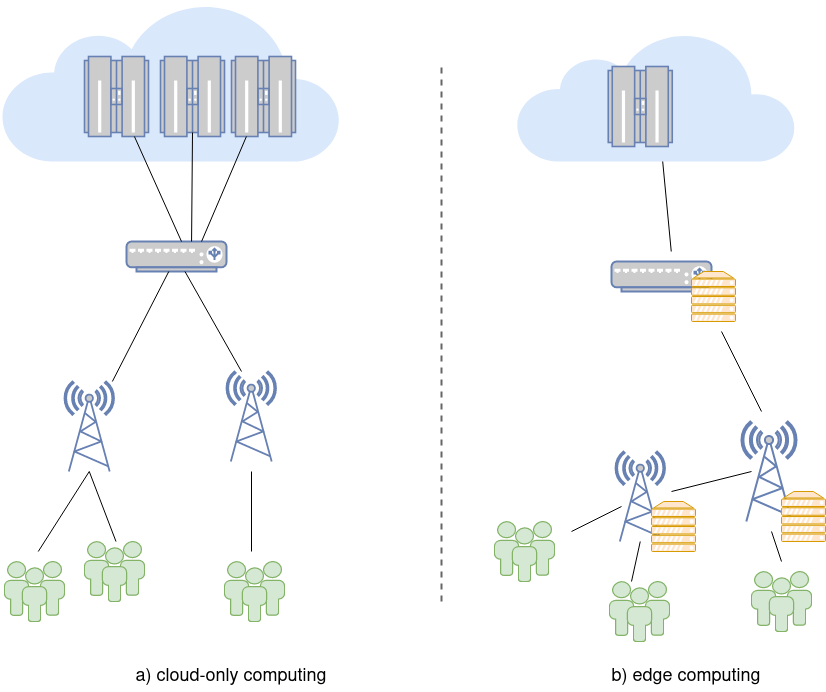
\includegraphics[width=12cm]{graphics/diagrams/edge_computing_example.png}
    \caption{An example of how in b) edge computing there are nodes interspersed throughout the network and close to clients, while in a) cloud computing all computation is centralized.}
    \label{fig:edge_comp_example}
\end{figure}

Edge computing enables a number of structural benefits that allow for the creation of new types of use-case and application.
Most notably, edge computing enables low latency, high bandwidth, computation offloading.
This can be used to improve application responsiveness, perform computations not possible on low-powered devices, or conserve energy on mobile devices by offloading complex computations to nearby edge nodes\cite{abbasMobileEdgeComputing2018b}.
Edge computing can also been seen as a way to transparently improve cloud computing, reducing the overall traffic in the network and making existing cloud applications more responsive by moving them closer to the user\cite{satyanarayananEmergenceEdgeComputing2017}.
Figure \ref{fig:edge_comp_example} shows the difference between edge and cloud computing in a simplified way.
In the example edge computing features computational nodes on \gls{ran}-towers, and thus much closer to the users.


This computing paradigm does, however, pose a challenge to existing frameworks and application architectures.
Given that computation resources are spread  farther throughout the network, the network infrastructure itself in edge computing is much more diverse\cite{shiEdgeComputingVisionChallenges2016}, potentially consisting of anything from the unreliable mobile network connection of a user's device to high bandwidth fiber networks between cloud data centers.
From both a hardware and software perspective, the computation hardware itself is more heterogeneous as well, requiring specific optimization mechanism to use resources in the most efficient way possible\cite{abbasMobileEdgeComputing2018b}.

\subsection{Serverless at the Edge}
Since serverless computing offers an abstraction layer on top of the actual infrastructure \cite{jonasCloudProgrammingSimplified2019}, and a key challenge of edge computing is that edge applications, at least up to now, have to be specifically crafted for their deployment scenario by developers\cite{shiPromiseEdgeComputing2016}.

With future \gls{ai} applications being dependent on edge computing to deliver their benefits to users via augmented reality, and smart city infrastructure\cite{rauschEdgeIntelligenceConvergence2019}, serverless offers an attractive abstraction layer to develop such \gls{ai} applications in an edge-native way.
Building on serverless as an abstraction layer for the application, the idea is that it will be able to jointly provide the benefits afforded by edge computing and serverless computing at the same time.
Functions are supposed to be deployed to nodes close to the users that rely on these functions, be scaled automatically, and routed efficiently, without any manual intervention from developers.

Achieving such a computing infrastructure would enable a host of new types of application, such as wearable cognitive assistance\cite{haWearableCognitiveAssistance2014}\cite{rauschPlatformSmartCityScale2021}, offloading \gls{ai} inference tasks from devices with low compute capability\cite{liEdgeAIOnDemand2020}, and analyzing video feeds in real time to improve public safety\cite{zhangEdgeVideoAnalytics2019}, for example to ensure face masks are worn where mandated\cite{wangWearMaskFastInbrowser2021}.

Open source serverless frameworks have been evaluated in terms of their performance in edge-scenarios, but in their current, unmodified state they lack the full set of capabilities needed to provide all the benefits edge computing offers\cite{paladeEvaluationOpenSource2019}.
While some of these serverless frameworks have been adapted to address the challenges posed by the edge computing environment, or to be better tailored to workloads related to \gls{ai}\cite{rauschServerlessPlatformEdge}, more of which will be discussed in the next chapter, overall there remain a lot of challenges for the universal practical application of serverless edge computing\cite{aslanpourServerlessEdgeComputing2021}.
Optimizing the performance of network bound workloads, for example, is one such challenge\cite{skippy}, and the one this thesis aims to address.



